\section{Download Sources}


\subsection{U-Boot Source}
U-Boot is the second stage boot loader used to load the the Linux kernel and root filesystem. For U-Boot to load the kernel, the kernel image needs to be wrapped with a U-Boot header. U-Boot is built with a \texttt{mkimage} utility which is used to wrap the kernel image. \texttt{mkimage} is also used to wrap file system images with U-Boot headers for loading. To build Linux images, U-Boot source needs to be downloaded and compiled to provide the \texttt{mkimage} utility binary. \\

\noindent
To download the U-Boot source needed to compile snickerdoodle Linux images, the following \texttt{git} command can be executed from the command line: \\

\begin{lstlisting}[style=text]
git clone https://github.com/krtkl/snickerdoodle-u-boot.git
\end{lstlisting}


\subsection{Linux Source}
The source required to configure and compile the Linux kernel for snickerdoodle can be downloaded using the following \texttt{git} command: \\

\begin{lstlisting}[style=text]
git clone https://github.com/krtkl/snickerdoodle-linux.git
\end{lstlisting}


\subsection{Checkout Stable Branch}
At the time of this document's publication, the current stable and supported kernel release for snickerdoodle is 3.14. The \texttt{sd-linux/3.14} branch of the snickerdoodle Linux kernel has been updated to include the necessary driver source to run the snickerdoodle peripherals (wireless, etc.). To switch the local repository to this branch, the following \texttt{checkout} command can be used: \\

\begin{lstlisting}[style=text]
git checkout sd-linux/3.14
\end{lstlisting}


\subsection{snickerdoodle Default kernel Configuration}

Before the kernel or any of the executables that are build 

\begin{lstlisting}
make ARCH=arm zynq_snickerdoodle_defconfig
\end{lstlisting}



\section{Build U-Boot}

\subsection{Generate Build Script Utilities}
U-Boot requires a utility that is normally built with the kernel. The device tree compiler (\texttt{dtc}) is used to compile device tree blobs from source and is called during the build process for U-Boot. Interestingly, building U-Boot requires a utility that is normally built with the kernel while the Linux kernel requires a utility that is normally built with U-Boot (\texttt{mkimage}). To avoid building a kernel image (can take quite a long time depending on host computer performance) just to access the \texttt{dtc} and still being required to recompile the kernel after U-Boot has been built, the utilities in the \texttt{scripts} directory (including \texttt{dtc}) can be compiled with the following invocation: \\

\begin{lstlisting}[style=text]
make ARCH=arm CROSS_COMPILE=arm-xilinx-linux-gnueabi- scripts
\end{lstlisting}

~\\
\noindent
After building the scripts within the Linux source repository, the path to the device tree compiler must be added to the \texttt{\$PATH} variable so that it is available to \texttt{make} when building U-Boot. After navigating to \textit{\bfseries snickerdoodle-linux $\rightarrow$ scripts $\rightarrow$ dtc}, the \texttt{\$PATH} variable can be updated as shown below: \\

\begin{lstlisting}[style=text]
cd scripts/dtc
export PATH=$PATH:$(pwd)
\end{lstlisting}

\subsection{Build U-Boot and \texttt{mkimage}}

After the device tree compiler has been built, U-Boot can be built from the it's top-level directory by invoking the following command: \\

\begin{lstlisting}[style=text]
make ARCH=arm CROSS_COMPILE=arm-xilinx-linux-gnueabi- 
\end{lstlisting}

~\\
\noindent
Just as with the device tree compiler, for \texttt{mkimage} to be callable from \texttt{make} during the kernel build process, it's parent directory must be added to \texttt{\$PATH}. The \texttt{mkimage} executable is built in the \texttt{tools} directory within the U-Boot source directory. By navigating to \textit{\bfseries snickerdoodle-u-boot $\rightarrow$ tools}, the \texttt{\$PATH} variable can be appended with the location of the \texttt{mkimage} utility. \\

\begin{lstlisting}
cd tools
export PATH=$PATH:$(pwd)
\end{lstlisting}

~\\
\noindent
To test that \texttt{mkimage} has been made available to be called by the system (and to debug possible conflicting installations of \texttt{mkimage}), \texttt{which} can be used to output the parent directory of the \texttt{mkimage} binary: \\

\begin{lstlisting}[style=text] which mkimage
/home/snickerdoodle/snickerdoodle-u-boot/tools/mkimage
\end{lstlisting}

~\\
\noindent
The above output shows the \texttt{mkimage} executable located in the directory that was added to \texttt{\$PATH} in the previous step.


\section{Configure Linux}

After the \texttt{mkimage} utility has been generated, the Linux kernel can be built for U-Boot. Before building, a configuration file (\texttt{.config}) must be produced to define the kernel build options. The default snickerdoodle configuration can be specified using \texttt{make}: \\

\begin{lstlisting}[style=text]
make ARCH=arm zynq_snickerdoodle_defconfig
\end{lstlisting}

~\\
\noindent
If additional configuration options are needed, the configuration can be edited using a variety of interfaces. \texttt{make} can be called to initiate the configuration interface using the following command: \\

\begin{lstlisting}[style=text]
make ARCH=arm <config_interface>
\end{lstlisting}

~\\
\noindent
Options for \texttt{<config\_interface>} are:


\margininfonote{Necessary libraries can be installed using \texttt{sudo apt-get install} commands along with the required libraries specified for the interface}


\begin{description}
	\item[\texttt{config}] - Text-based interface
	\item[\texttt{menuconfig}] - Text-based interface with hierarchical menus, radiolists and interactive assistance. This option allows incremental saving of changes. (ncurses must be installed: \texttt{libncurses5-dev})
	\item[\texttt{nconfig}] - Text-based menus (curses must be installed: \texttt{libcdk5-dev})
	\item[\texttt{xconfig}] - QT/X-windows interface (QT is required: \texttt{qt4-dev-tools})
	\item[\texttt{gconfig}] - Gtk/X-windows interface (GTK is required)
\end{description}


\begin{figure}
	\centering
	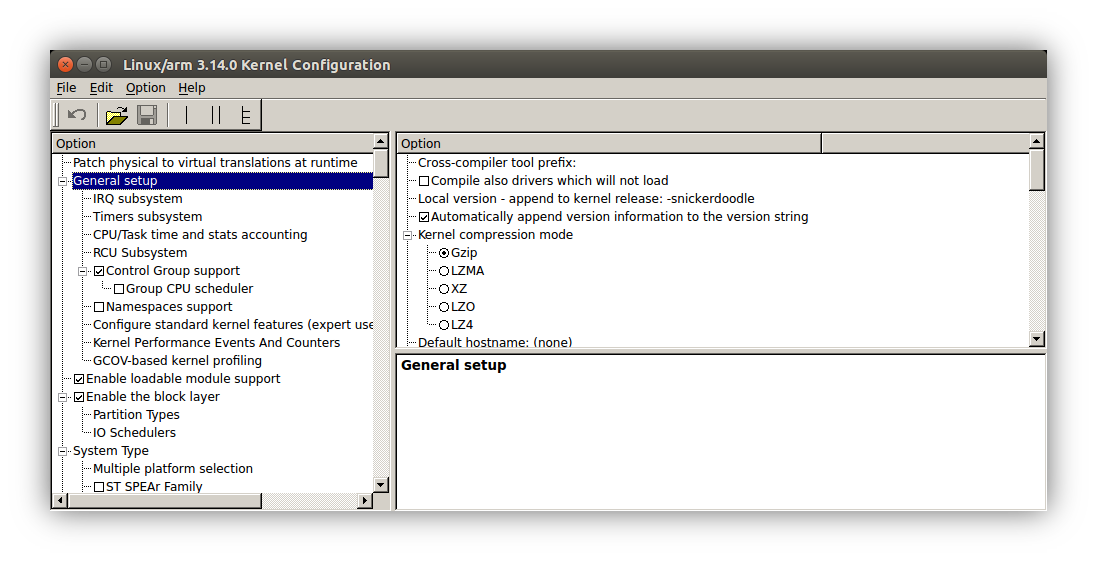
\includegraphics{images/xconfig.png}
	\caption{QT/X-Windows Configuration Interface (\texttt{xconfig})}
	\label{fig:xconfig}
\end{figure}


\noindent
\figref{fig:xconfig} shows the QT based configuration interface that can be used to configure Linux build options. \\


\section{Building Linux}

The next and final step for building the Linux kernel is the build process itself. While building, the build components will be output to the console. A clean build can take quite a while. To build the Linux kernel with the necessary U-Boot header, the \texttt{uImage} argument should be specified. The following command will begin the build process: \\

\begin{lstlisting}
make ARCH=arm CROSS_COMPILE=arm-xilinx-linux-gnueabi- LOADADDR=0x8000 uImage
\end{lstlisting}


~\\
\noindent
The build process will output messages for each compilation step. After the final build step is complete, a set of messages similar to the following will appear (note the output image path on the last line): \\

\begin{lstlisting}[style=text]
  Kernel: arch/arm/boot/zImage is ready
  UIMAGE  arch/arm/boot/uImage
Image Name:   Linux-3.14.0-snickerdoodle-00004
Created:      Fri Dec 11 16:34:56 2015
Image Type:   ARM Linux Kernel Image (uncompressed)
Data Size:    4145568 Bytes = 4048.41 kB = 3.95 MB
Load Address: 00008000
Entry Point:  00008000
  Image arch/arm/boot/uImage is ready

\end{lstlisting}


\subsection{Build and Install kernel Modules}

The kernel modules, if any have been specified by the Linux configuration, can be built by invoking: \\

\begin{lstlisting}[style=text]
make ARCH=arm CROSS_COMPILE=arm-xilinx-linux-gnueabi- modules
\end{lstlisting}

~\\
\noindent
After building the kernel modules, they can be installed into a root file system by calling: \\

\begin{lstlisting}[style=text]
make ARCH=arm INSTALL_MOD_PATH=<path_to_rootfs> modules_install
\end{lstlisting}



%
%~\\
%\noindent
%For example, a \textit{ROOTFS} partition that has been mounted at \texttt{/media/ROOTFS}: \\
%
%\begin{lstlisting}[style=text]
%make ARCH=arm INSTALL_MOD_PATH=/media/ROOTFS modules_install
%\end{lstlisting}






